\documentclass{article}
\usepackage{neurips_2026}
\usepackage[utf8]{inputenc}
\usepackage[T1]{fontenc}
\usepackage{hyperref}
\usepackage{url}
\usepackage{booktabs,array}
\usepackage{amsmath,amssymb,amsthm}
\usepackage{graphicx}
\usepackage{microtype}
\usepackage{xcolor}
\newtheorem{proposition}{Proposition}
\newtheorem{corollary}{Corollary}
\newcommand{\tr}{\operatorname{tr}}
\newcommand{\E}{\mathbb{E}}
\newcommand{\R}{\mathbb{R}}
\DeclareRobustCommand{\artifact}[1]{\path{#1}}
\makeatletter
\let\tableinput\@@input
\makeatother
\title{Predicting Held-Out Benchmark Scores from Few Whole Benchmarks:\\A Descriptive Study of Coverage, Selection, and Dependence}
\author{Anonymous Authors}
\begin{document}
\maketitle
\begin{center}
\emph{Research draft; not submitted or accepted.\\The official-template footer is formatting boilerplate, not a status claim.}
\end{center}

\begin{abstract}
Can a few whole-benchmark measurements help predict a new model's other scores? We study standard Gaussian conditional prediction and training-only benchmark selection using incomplete public score tables, with disjoint acquisition candidates and fixed audit targets. A 279-model, 62-task MTEB source matrix supports original experiments on only eight candidate and four audit tasks per split. The prospective feasibility gate passes just one of five organization holdouts, below the required three; all empirical findings are therefore descriptive. Across all five original splits and budgets $k=1,2,4$, residual-trace greedy selection has normalized mean squared error 0.357 versus 0.421 for random acquisition with the same predictor: a 15.1\% relative reduction, with a conditional descriptive 95\% interval of [9.7,20.6]\%. A post-audit 61-task incomplete-panel sensitivity gives 0.239 versus 0.296, but audit-aware, correlation, and mean-filled-covariance comparators have lower point estimates. Original OpenLLM splits share revision keys; a metadata-connected exploratory analysis removes recorded key overlap, not all ancestry dependence. We preserve these failures and qualify uncertainty, budget selection, and missingness results. Standard Gaussian identities explain why measured-coordinate removal is not fixed-target transfer and why no universally useful measurement budget follows. No new algorithm, greedy optimality, full-suite recovery, or confirmed superiority is claimed.
\end{abstract}

\section{Introduction}\label{sec:intro}
Evaluating every model on every benchmark is often impractical. Historical score tables suggest a narrower possibility: measure a few benchmarks for a previously held-out model and use relationships estimated from older models to predict other scores. Here a label is an entire benchmark score, not an example or prompt. Equal label counts are an accounting convention, not measured evaluation costs. Our primary domain is embedding models, whose heterogeneous evaluation tasks make broad score extrapolation particularly uncertain \citep{muennighoff2022mteb}.

A central evaluation difficulty is distinguishing useful transfer from the mechanical benefit of no longer predicting a measured coordinate. If a policy measures a difficult benchmark and removes it from its error calculation, error can decrease even when the measurement tells us nothing about any other benchmark. We therefore evaluate on fixed, disjoint audit tasks that no policy may acquire. All methods within a condition see the same rows, available candidates, and target cells at each budget. A changing-target deployment error is reported only as a diagnostic, not as a fair head-to-head selector comparison.

The intended test was more ambitious than the available evidence permits. Only one of five original MTEB organization holdouts meets the predeclared dense-cohort feasibility thresholds; the required minimum was three. We retain all five seeds rather than promote the feasible split, random-row analysis, or another dataset to confirmation. Original OpenLLM organization splits additionally share nonempty revision SHA keys across training and test partitions. Later wider-panel and metadata-connected analyses are versioned sensitivities on reused data, not pristine retests. These restrictions govern every empirical statement in this paper.

The study contributes an auditable descriptive comparison, not an acquisition algorithm. First, it separates ingestion breadth from evaluated target support and documents feasibility, dependence, and exposure limitations. Second, it compares standard selectors and inductive predictors under equal whole-benchmark budgets, validation-only tuning, and paired uncertainty. Third, it gives complete standard Gaussian derivations and explicit boundary examples to clarify what covariance-based design does and does not justify. The resulting evidence suggests useful conditional score relationships in the observed cohorts, but neither a unique winning method nor a universal small budget.

\section{Related work}\label{sec:related}
\paragraph{Benchmark heterogeneity.}
MTEB spans different embedding tasks and metrics, rather than interchangeable accuracy measurements \citep{muennighoff2022mteb}. Its inspected analyses emphasize task-dependent model rankings and inherited training-data overlap. We use a pinned results snapshot, not the original paper's historical model or dataset counts, and do not interpret a selected similarity-heavy panel as representative embedding quality.

\paragraph{Item compression versus whole-benchmark acquisition.}
\citet{maiapolo2024tinybenchmarks} combine representative item selection with item-response prediction and bias--variance correction. \citet{kipnis2024metabench} use information-based item filtering and calibrated score reconstruction, including joint information from multiple reduced benchmarks. Those approaches use item-level responses; our input contains only aggregate whole-task scores. Their example budgets, absolute errors, and information regimes are consequently not directly comparable to ours. We do not reproduce them or imply that whole-benchmark acquisition supersedes item compression.

\paragraph{Capability-based prediction.}
\citet{ruan2024observationalscaling} predict downstream performance from measured benchmark-derived capabilities, with training-only preprocessing in the inspected protocol. \citet{maiapolo2024sloth} model skills using size, tokens, and family offsets, with observed anchors from a target family. We instead infer one held-out row from its acquired scores without fitting jointly with other test rows or assuming resource metadata. Organization/component holdouts here are not family-lineage holdouts. This literature review is deliberately restricted and nonexhaustive: only selected sections of these five supplied papers were read. We make no priority or exhaustive novelty claim; exact access and reading scope are recorded in Appendix~\ref{app:sources}.

\section{Protocol, data, and evaluation}\label{sec:protocol}
\subsection{Stages and feasibility}
The internal plan specifies: pinned acquisition and schema QC; mask/metadata-defined cohorts and feasibility gates; standard-estimator checks and validation tuning; frozen paired evaluation; training-missingness stresses; and optional transfer/reporting. Success means an honest held-out error comparison, including negative results, rather than a positive method result. The dense MTEB ladder tries candidate/audit counts $(16,8)$, $(10,6)$, then $(8,4)$ using training coverage and held-out masks only. A split requires at least 60 usable training rows/15 groups, 20 complete validation rows/5 groups, and 30 complete test rows/8 groups. At least three of five preset organization splits must pass before confirmatory interpretation is allowed.

\begin{table}[t]
\centering
\caption{Original MTEB organization holdouts. Counts are rows/groups; panels contain eight candidates and four audit tasks. The study-level $\geq3/5$ gate fails, so even seed 37 is descriptive. Source: \artifact{artifacts/cohort_counts.csv}.}
\label{tab:gate}
\begin{tabular}{rrrrl}
\toprule
Seed & Training & Validation & Dense test & Local gate \\
\midrule
\tableinput{../artifacts/paper_gate.tex}
\bottomrule
\end{tabular}
\end{table}

Table~\ref{tab:gate} shows the failure without dropping inconvenient seeds. Final summaries equally weight all five preset split means, a descriptive fallback rather than the planned accepted-split confirmatory estimand. Internal protocol hashes are provenance records, not externally timestamped preregistration. Schema inspection materialized two OpenLLM source rows including scores before locking; no test-based tuning was found in the code audit, but an exposure-free historical test lock is not established.

\subsection{Canonical data and quality control}
MTEB results are pinned to commit \texttt{6dabbcc68c28ea5f180ce7df79347b3ca9cc6383}. Streaming the archive finds 547 directories with results, retaining a $279\times62$ English-task matrix with 9,882 observed cells (57.13\%). Extraction selects one revision per model by coverage, one finite English test \texttt{main\_score} per task, and a modal dataset revision per task. Accepted values lie in $[-1,1]$, including correlation metrics; missing or ambiguous values remain missing, never fabricated zero targets. There are no duplicate retained model/task provenance records or unknown retained dataset revisions. This is not full harmonization of evaluator versions, prompts, or configurations: source \texttt{mteb\_version} was not retained. Training duplicate rows were counted but not removed, a protocol deviation.

OpenLLM uses the pinned \texttt{open-llm-leaderboard/contents} revision \texttt{9c09a7cae43334062a82cb164f2ef255013dafa2}. Precision/fullname selection retains 4,497 complete rows from 4,576 records and six raw proportion scores, excluding aggregate/display scores. A preliminary erroneous division by 100 was corrected at schema inspection before fitting or prediction. Original organization splits have 4--6 shared nonempty training/test SHA values per seed. Their errors are retained as dependent-row descriptions; independence interpretation is quarantined. Appendix~\ref{app:assets} gives source URLs and licensing restrictions.

\subsection{Splits, task roles, and distinct estimands}\label{sec:support}
Seeds are 11, 23, 37, 53, and 71. These are repeated train/validation/test holdouts, not disjoint five-fold cross-validation. Shuffled whole groups are allocated by greatest proportional row deficit toward 60/20/20; unknown organizations are pooled. Organization names are imperfect dependence proxies. A secondary random-row regime has different panels/cohorts and cannot isolate a causal effect of organization shift.

For original MTEB, tasks require at least 40 training observations, 60\% coverage, and nonconstant training scores. Permanent hash roles separate candidates $C$ from audit targets $T$; coverage/hash ordering selects the panels without the planned task-type round-robin. Every original panel has 12 tasks, not 62. Across the five organization splits, the union is 15 panel tasks and six audit tasks. Dense validation/test rows observe the entire panel; incomplete training rows with at least two panel cells are retained. Original native cohorts require at least four available candidates and two observed audit targets, with fixed eligibility through $k=4$. Their test sizes are 38,48,37,40,47; OpenLLM uses three candidates/three audit tasks and native $k\leq2$.

Two post-audit sensitivities have separate estimands. \emph{Wide-native MTEB} keeps the organization partitions and task roles but removes the 60\% coverage and panel-size caps, retaining the 40-observation rule. All splits have 49 candidates and 12 audits, a 61-task panel; each test row has only 4--12 observed audit targets. Validation/test eligibility requires eight candidate and four audit observations; test counts are 47,44,47,43,46. This is broader observed-support prediction, not full-suite ground truth. \emph{Alias-connected OpenLLM} unions normalized organizations with nonempty model-SHA and Base Model keys before partitioning. It has zero recorded cross-partition SHA/base/component overlap, but metadata cannot recover all ancestry. A large connected component makes seed 71 grossly imbalanced: 3,161/4,497 (70.3\%) rows are test, with only 1,002 training rows. A connected component contains 2,890 rows (64.3\% of the dataset), including 91.4\% of seed 71's test rows; conditional bootstrap percentiles do not establish population coverage under this concentration. Neither sensitivity restores confirmation or constitutes a clean new sample.

\subsection{Loss, contrasts, and uncertainty}\label{sec:uncertainty}
Let $F_i\subseteq C$ and $T_i\subseteq T$ be the fixed observed candidate and audit supports of row $i$. All policies use these same supports. With means $\mu_t$ and scales $s_t$ fitted only on observed training cells, define $z_{it}=(x_{it}-\mu_t)/s_t$ and
\begin{equation}
 \ell_i(k)=\frac{1}{|T_i|}\sum_{t\in T_i}(\widehat z_{it}(A_i(k))-z_{it})^2,\qquad A_i(k)\subseteq F_i.
 \label{eq:loss}
\end{equation}
NMSE averages this per-row loss; native support gives equal weight to observed targets within a row, not equal global task weight. Core loss $L$ averages $k\in\{1,2,4\}$ for MTEB or $\{1,2\}$ for OpenLLM within each split, then equally averages five split means. This is not a logarithmic area under a curve. We report $\Delta=L_{\mathrm{policy}}-L_{\mathrm{random}}$ and $I=1-L_{\mathrm{policy}}/L_{\mathrm{random}}$. Raw RMSE is the square root of equal-split mean per-row raw MSE, not the mean of row RMSEs; MTEB raw units mix metrics and are not uniformly accuracy percentages.

Intervals use 2,000 paired cluster-bootstrap draws and the 2.5/97.5 percentiles. Organizations (metadata components for corrected OpenLLM) are sampled once jointly across all repeated appearances, carrying methods and budgets together and recomputing equal-split estimates. Empty-split draws are excluded. Tasks, anchor paths, and repeated split appearances are not independent observations. These conditional descriptive intervals hold trained pipelines, selected cohorts, and the original 50-path bank fixed; they omit full refitting, source, selection, and random-bank uncertainty. There are no superiority tests, $p$-values, or multiplicity-corrected significance claims. Secondary comparisons remain descriptive rather than being interpreted through unadjusted interval exclusion.

\section{Standard predictors and acquisition policies}\label{sec:method}
\subsection{Training-only estimators and matched comparisons}
For standardized training data, pairwise covariance uses overlap-centered pairs with at least 20 shared observations; unsupported off-diagonals are set to zero. Symmetrization, eigenvalue clipping at $10^{-8}$, and diagonal renormalization produce $\widehat\Sigma_{\mathrm{PSD}}$. The fitted covariance is
\begin{equation}
 \widehat\Sigma_\lambda=(1-\lambda)\widehat\Sigma_{\mathrm{PSD}}+\lambda\operatorname{diag}(\widehat\Sigma_{\mathrm{PSD}}),\quad
 \widehat z_T=\widehat\Sigma_{TA}(\widehat\Sigma_{AA}+10^{-6}I)^{-1}z_A.
 \label{eq:fit}
\end{equation}
Implementation uses solves, not explicit inverses. The ridge is numerical stabilization, not a fitted observation-noise model. One $\lambda\in\{0,.1,.3,.6,.9,1\}$ is selected on mean validation audit loss across random paths and core budgets, and shared by Gaussian selectors. Ties within $10^{-4}$ favor stronger shrinkage. No fitting or centering uses other held-out rows.

The bounded low-rank baseline minimizes masked reconstruction error plus $\alpha(\|U\|_F^2+\|B\|_F^2)$ by alternating ridge solves. Ranks are $\{1,2,4,8\}$ capped by task count, and $\alpha\in\{.01,.1,1\}$, selected by the same validation criterion. Three fixed starts (101,202,303) have at most 200 iterations and relative objective tolerance $10^{-5}$; predictions are averaged across starts. A new row solves its own ridge latent regression from acquired labels using training loadings only. Selected original MTEB seeds 11 and 37 have all three starts capped; seed 53 has one capped start. Thus the comparison is against a fixed-compute baseline, not a converged optimum.

\paragraph{Selectors and ablations.}
Residual greedy (\texttt{greedy\_deploy}) minimizes the conditional covariance trace on all panel coordinates not yet acquired. Audit greedy minimizes it on fixed $T$ only. These paths depend on training covariance and candidate availability, not acquired score values. High variance ranks original-unit training variance and is unit-dependent. Correlation coverage greedily maximizes $\sum_{t\in T_i}\max_{a\in A}\widehat\Sigma_{\lambda,ta}^{\,2}$, using entries of the fitted, PSD-repaired, shrunk unit-diagonal matrix, not a separate Pearson-correlation fit; it is audit-aware. Random uses 50 fixed nested permutation paths, reusing paths across relevant comparisons and averaging \emph{losses}, not predictions. Low-rank predictors use identical random or residual-greedy anchors to isolate imputation; D-optimal factor selection is a separate full baseline. Mean prediction spends zero labels, even when displayed as a flat curve at larger $k$. No-shrinkage and mean-filled covariance use audit-greedy selection, so their direct comparison is to audit greedy, not an isolated residual-selector ablation. Appendix~\ref{app:details} specifies the remaining details.

For native cohorts, residual greedy still optimizes the \emph{full panel}, including historically unavailable coordinates; reported deployment error scores only observed unacquired coordinates. This objective/support mismatch is not an observed-support-aligned acquisition rule. Fixed-audit NMSE nevertheless remains a paired evaluation of the implemented policy. Deployment NMSE changes targets with the selected set and is not fair fixed-target evidence (Appendix~\ref{app:target}).

\subsection{Gaussian interpretation and boundaries}\label{sec:theory}
These are standard identities under a known finite population covariance $\Sigma\succ0$, $X\sim N(0,\Sigma)$, unit diagonal, exact observations $X_A$, and fixed disjoint $A\subseteq C$ and nonempty $T$. Write $U=D\setminus A$ and $V=\Sigma_{UU}-\Sigma_{UA}\Sigma_{AA}^{-1}\Sigma_{AU}$. The conditional mean minimizes squared error, with fixed-target Bayes sum-risk $R_T(A)=\tr V_{TT}$. Revealing $j\in C\setminus A$ reduces risk by
\begin{equation}
 \Delta_T(j\mid A)=\frac{\|V_{Tj}\|_2^2}{V_{jj}},\qquad
 \Delta_{\mathrm{dep}}(j\mid A)=V_{jj}+\sum_{u\in U\setminus\{j\}}\frac{V_{uj}^2}{V_{jj}}.
 \label{eq:gains}
\end{equation}
The second expression is for sum-error over all remaining coordinates and includes self-removal. For independent unit-variance candidate/target coordinates, measuring the candidate reduces deployment risk $2\to1$ but leaves target risk $1\to1$. The trace of the fully conditioned old covariance already includes zero measured-coordinate variance under exact observation; subtracting it again is incorrect.

A Gaussian residual is independent of the measured values, so these gains depend on indices, not score values. Under a fixed budget and value-independent feasible sets, even a nonanticipating value-adaptive policy cannot beat the best predetermined subset in Bayes risk. This does \emph{not} establish greedy optimality or submodularity: a positive-definite suppressor example has marginal gain $0$ before another observation and $1/12$ afterward. If $\Sigma$ has independent target/candidate blocks, even acquiring all candidates leaves risk $|T|$; no covariance-uniform budget guarantees any positive fractional target-risk reduction. Proofs, the precise quantifiers, and a strict objective-ranking reversal appear in Appendix~\ref{app:proofs}. Estimated covariance, natural missingness, non-Gaussian scores, and numerical ridge do not inherit population-risk or predictive-calibration guarantees.

\section{Descriptive results}\label{sec:results}
\subsection{Fixed-audit comparisons}
\begin{table}[t]
\centering
\caption{Core fixed-audit NMSE (lower is better), equally weighted over five organization/component split means. All 11 methods are retained; columns describe different estimands, not a pooled comparison. Original MTEB uses eight candidates/four audits; wide MTEB uses observed subsets of 12 audits; OpenLLM is the post-audit connected sensitivity. All results are descriptive. Full conditional intervals and quarantined original OpenLLM results are in Appendix~\ref{app:tables}. Source: \artifact{artifacts/summary.csv}.}
\label{tab:main}
\begin{tabular}{lrrr}
\toprule
Method & Original MTEB & Wide MTEB & Connected OpenLLM \\
\midrule
\tableinput{../artifacts/paper_compact.tex}
\bottomrule
\end{tabular}
\end{table}

Original MTEB residual greedy gives core NMSE 0.357 versus 0.421 for the same-imputer random policy (Table~\ref{tab:main}). The paired difference is $-0.0636$ with descriptive interval $[-0.0925,-0.0409]$; relative reduction is 15.1\% [9.7,20.6]\% (Table~\ref{tab:contrasts}). Its split-wise point losses are below random in all five seeds, but the study-level feasibility failure still prevents confirmation. Audit greedy and correlation coverage give 0.372 and 0.369; these results do not identify a uniquely superior selector. Residual-anchor factors give 0.361, close to Gaussian prediction, whereas random-anchor factors give 0.432 and D-optimal factors 0.417. Nonconvergence weakens any claim against optimized low-rank prediction.

\begin{table}[t]
\centering
\caption{Residual greedy versus the same Gaussian imputer with random acquisition. Brackets are paired conditional descriptive 95\% intervals, not multiplicity-corrected superiority evidence. Original OpenLLM is retained but quarantined for independence interpretation. Core budgets and averaging are defined in Section~\ref{sec:uncertainty}. Sources: \artifact{artifacts/summary.csv}, \artifact{artifacts/contrast_table.tex}.}
\label{tab:contrasts}
\begin{tabular}{lrr}
\toprule
Condition & Absolute NMSE difference $\Delta$ & Relative reduction $I$ (\%) \\
\midrule
\tableinput{../artifacts/paper_contrasts.tex}
\bottomrule
\end{tabular}
\end{table}

Wide-native MTEB gives residual greedy 0.239 versus random 0.296, a 19.3\% [14.3,24.8]\% reduction, but audit greedy (0.228), correlation coverage (0.223), and mean-filled covariance (0.217) have lower point estimates. No-shrinkage gives 0.225 versus audit greedy 0.228, so shrinkage is not universally beneficial. Conversely, original audit-greedy shrinkage (0.372) and no-shrinkage (0.374) are close. These comparisons motivate an objective- and cohort-dependent interpretation rather than a universal method ranking. Different panels, target availability, and training scales preclude interpreting the lower wide-cohort loss as a controlled improvement over the original cohort.

Original OpenLLM gives 0.469 versus 0.530 but cannot support independent unseen-revision transfer. Connected OpenLLM gives 0.429 versus 0.500, a 14.2\% [11.6,16.1]\% relative reduction. Residual and audit greedy coincide at reported precision, while correlation coverage gives 0.435 and factor D-optimal design 0.650. The latter is a negative comparison: its core loss exceeds random, rather than providing a general design advantage. Zero recorded-key overlap does not remove unknown ancestry or the seed-71 imbalance, and neither analysis rescues the original MTEB gate.

\begin{figure}[t]
\centering
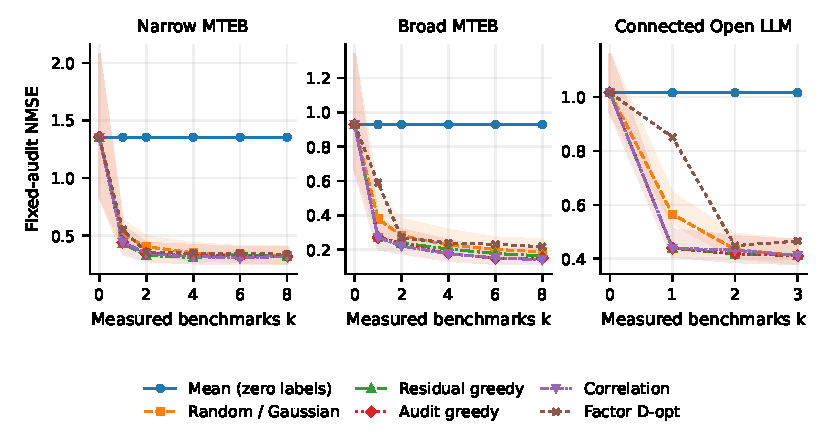
\includegraphics[width=\linewidth]{../artifacts/budget_curves.pdf}
\caption{Fixed-audit error versus acquired whole benchmarks. Shading shows conditional descriptive 95\% intervals for random and audit greedy only. Mean prediction spends zero labels despite its flat display. The three panels are distinct coverage-conditioned estimands; none establishes full62 recovery or independent family generalization. Source: \artifact{artifacts/budget_curves.pdf}, generated by \artifact{src/analyze.py}.}
\label{fig:budgets}
\end{figure}

\subsection{Budgets, robustness, and numerical checks}
Figure~\ref{fig:budgets} shows fixed-budget curves without choosing the best test $k$. The validation-only global rule chooses the smallest $k$ within one organization-bootstrap SE of the minimum validation loss, including $k=0$; it is not per-model risk calibration. For original MTEB residual greedy, selected budgets in seed order are $(2,2,2,1,1)$; random selects $(4,4,6,2,2)$, audit greedy $(2,4,4,1,1)$, and correlation $(6,2,4,1,4)$. At those budgets residual-greedy dense-test NMSEs are $(.400,.223,.218,.304,.646)$ and random losses are $(.505,.274,.171,.360,.535)$: fewer labels do not uniformly give lower loss. Original OpenLLM residual/audit/correlation select $k=1$ in all seeds, while random selects $k=2$. These are original dependent-row results, not budgets established for the corrected sensitivity. Selected-budget native results are unavailable when a frozen budget exceeds the native ceiling; we do not cap or substitute them. Complete records are in \artifact{artifacts/validation_budgets.csv}.

\begin{figure}[t]
\centering
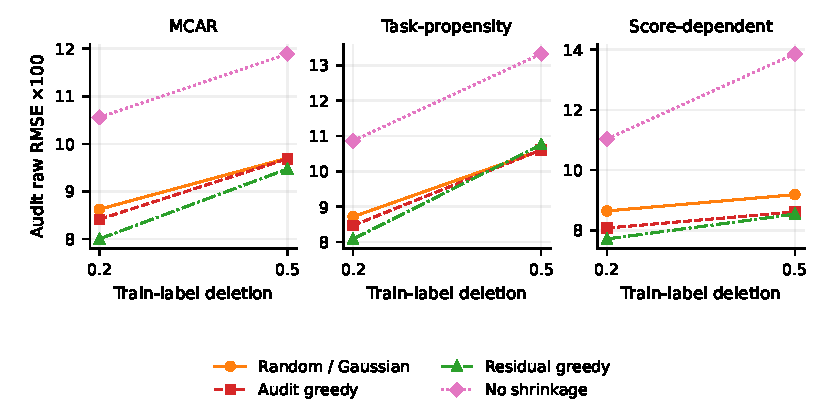
\includegraphics[width=\linewidth]{../artifacts/missingness.pdf}
\caption{Training-only label deletion, original MTEB organization seeds 11,37,71; core budgets $1,2,4$, fixed dense test targets. Raw RMSE is shown because retained-training standardization changes with deletion. The vertical scale is raw error multiplied by 100, not uniformly accuracy percentage points. Lines are point estimates, not interval bands. Source: \artifact{artifacts/missingness.pdf}; conditional intervals are in \artifact{artifacts/summary.csv}.}
\label{fig:missing}
\end{figure}

Training deletion uses MCAR, task-propensity, and explicitly synthetic high-score-dependent mechanisms at 20\%/50\%, recomputing preprocessing, fitting, and validation tuning on retained labels only. Figure~\ref{fig:missing} shows deterioration and a reversal: at 50\% propensity deletion, residual greedy raw RMSE is 0.1076 versus random 0.1060, with NMSE 1.152 versus 1.137. No-shrinkage is especially unstable under deletion, reaching raw RMSE 0.1386 in the 50\% score-dependent condition. These secondary stresses cover six Gaussian/mean variants and three seeds, not low-rank robustness or a causal correction for real missingness. Historically absent scores still have no ground truth.

The original native MTEB core losses are 0.303 (residual) versus 0.348 (random); random-row dense losses are 0.313 versus 0.437. Their differing panels and coverage support make these contextual, not independent replications. Original OpenLLM native/dense cohorts coincide at common budgets because all six retained scores are observed. Appendix~\ref{app:tables} reports split heterogeneity and original transfer results rather than silently removing them.

A labelled synthetic check draws 100,000 samples from one seven-dimensional Gaussian. Across $k=0,1,2,3,4$, empirical target losses agree with known-covariance conditional traces to within about 1.3 Monte Carlo SEs (Appendix~\ref{app:synthetic}). This is only an implementation/identity check. On real MTEB seed 11 at $k=2$, residual-greedy trace risk is 0.288 versus observed NMSE 0.400; at seed 37 it is 0.323 versus 0.218. Traces are not calibrated predictive bounds.

The original random-bank Monte Carlo SE exceeds the predeclared 1\% trigger (organization splits: roughly 1.2--2.7\% for MTEB, 1.6--2.4\% for OpenLLM). A second independent 50-path bank, evaluated as sensitivity only, changes original MTEB split losses by $-1.7$\% to $+4.5$\%, wide MTEB by $-5.6$\% to $+6.5$\%, original OpenLLM by $-2.9$\% to $+2.7$\%, and connected OpenLLM by $-4.1$\% to $+2.5$\%. We retain original-bank headlines and conditional intervals; the second bank neither replaces their means nor creates a new confirmation. Sources are \artifact{artifacts/random_bank_mc.csv} and \artifact{artifacts/random_bank_sensitivity.csv}.

\section{Discussion and limitations}\label{sec:discussion}
\paragraph{What the evidence supports.}
Standard conditional prediction can exploit relationships among observed benchmark scores in these coverage-conditioned cohorts. Fixed audit targets make this narrower claim interpretable without crediting target removal. The relative random-policy comparisons coexist with simple competitive comparators, negative D-optimal results, and missingness reversals. A practical takeaway is to match the selection objective to the fixed prediction support and validate simple selectors before increasing predictor complexity; these data do not show that sophisticated design uniformly pays off. These observations favor careful evaluation design over a claim of algorithmic novelty or uniformly superior selection. There is no universally validated $k$, no score-adaptive acquisition benefit demonstrated, and no measured benchmark-runtime saving.

\paragraph{What remains unresolved.}
The failed feasibility gate, selected panels, informative historical reporting, repeated organizations, unharmonized evaluator details, and unavailable true scores on unreported cells limit external validity. Organization splitting is not family splitting; recorded-key separation is not ancestry independence. The corrected OpenLLM component imbalance further limits equal-split interpretation. Intervals exclude refitting, source uncertainty, and random-bank integration; validation is reused for tuning and the budget heuristic. Internal hashes do not establish historical sealing, and schema-head score exposure prevents claiming a pristine test history. Capped factor fits and omitted feasible complete-row covariance, wrong-objective diagnostic, standardized-variance tie reference, availability stress, category breakdown, chronological tests, and predictive interval calibration limit comparison completeness. Appendix~\ref{app:audit} preserves the deviation ledger. No favorable test result repairs these restrictions.

Future evidence should come from a genuinely untouched cohort with explicit revision/component separation, adequate fixed-target coverage, sealed fitted choices, converged bounded baselines, and measured benchmark-specific costs. A native-support-aligned selector first needs synthetic/training/validation contract tests; changing it now would not retroactively repair the evaluated policy. Full-suite claims require corresponding ground truth, not merely a wider source matrix.

\subsection{Broader impacts, assets, and automated research}\label{sec:ethics}
Score prediction may lower the barrier to exploratory comparison and help prioritize direct evaluations. It can also hide benchmark blind spots, suppress evidence of specialized failures, and encourage overconfidence about safety or underrepresented capabilities. A low average score error is not a safety certificate: safety-critical, fairness-sensitive, or out-of-domain decisions require direct evaluation and appropriate domain checks. No new human-subject study, crowdsourcing, pretrained model, or benchmark item generation was conducted.

MTEB result metadata specify CC0-1.0; upstream models and benchmark datasets have separate licenses. The OpenLLM score-table license remains unspecified; model Hub licenses are not a substitute. We do not claim permission to redistribute its raw source or row-level derivatives, and restrict distribution to code, provenance, and aggregate research summaries. Full existing-asset license compliance cannot be certified. The separately linked ethics code was not independently reviewed under the restricted access protocol; this is not a blanket certification of conformity.

\paragraph{LLM/agent disclosure.}\label{sec:agents}
Autonomous LLM agents participated in research design, coding, auditing, analysis, and manuscript drafting, not merely language editing. Citations and empirical claims are grounded in the inspected local evidence, but agent participation is not independent human validation. No LLM-as-judge target is used, and the numerical experiments require no foundation-model inference, GPU, or paid API. Exact agent-model/API cost accounting was not recorded; the CPU-only claim describes the numerical benchmark-score experiments.

\section{Conclusion}\label{sec:conclusion}
This study reports a descriptive, standard-method evaluation of predicting fixed audit scores from a few whole benchmarks. It retains a failed MTEB feasibility gate and quarantines original OpenLLM independence claims, while separating broader-support and metadata-connected sensitivities. Residual greedy improves on the stored random bank in the reported core averages, but simple comparators remain competitive and shrinkage and selection benefits depend on the condition. The principal limitation is the coverage- and dependence-conditioned evidence, not a missing universal algorithmic guarantee. Direct evaluation on new, adequately covered, independently audited cohorts is needed before stronger accuracy, budget, or cost claims.

\label{maintextend}
\clearpage
\bibliographystyle{plainnat}
\bibliography{references}
\clearpage
\appendix

\section{Complete Gaussian derivations and boundary constructions}\label{app:proofs}
These statements restate the standard identities and constructions in \artifact{theory.md}; they are not mathematical novelty claims or real-data guarantees. All dimensions are finite. Let $D=\{1,\ldots,d\}$, $X\sim N_d(0,\Sigma)$, $\Sigma=\Sigma^\top\succ0$, $\operatorname{diag}\Sigma=\mathbf1$, $\varnothing\ne T\subset D$, $C\subset D\setminus T$, and $A\subseteq C$. Observations are exact coordinates $X_A=x_A$ and loss is target \emph{sum} squared error. Initially observed coordinates also belong to $C$; no extra side information is assumed. Set $U=D\setminus A$ and, for nonempty $A$,
\begin{equation}
 m_U=\Sigma_{UA}\Sigma_{AA}^{-1}x_A,\qquad
 V^{(A)}=\Sigma_{UU}-\Sigma_{UA}\Sigma_{AA}^{-1}\Sigma_{AU}.
 \label{eq:schur}
\end{equation}
For $A=\varnothing$, set $m=0$, $V^{(A)}=\Sigma$. Principal submatrices are positive definite, so the inverse exists. For nonzero $z\in\R^{|U|}$ and $w=-\Sigma_{AA}^{-1}\Sigma_{AU}z$,
\begin{equation}
 z^\top V^{(A)}z=(w,z)^\top\Sigma_{(A,U),(A,U)}(w,z)>0.
 \label{eq:pd}
\end{equation}
Thus $V^{(A)}\succ0$ and every eligible scalar denominator is positive. Empty-set conventions avoid an inverse on no coordinates; an exhausted candidate pool requires no further action.

\begin{proposition}[Conditional prediction and risk]\label{prop:prediction}
Under the preceding assumptions, the conditional mean $m_T(A,X_A)$ uniquely minimizes fixed-target squared error up to almost-sure equality among measurable finite-risk predictors. Its conditional and unconditional Bayes risks are
\begin{equation}
 R_T(A)=\tr V^{(A)}_{TT}
 =\tr\bigl(\Sigma_{TT}-\Sigma_{TA}\Sigma_{AA}^{-1}\Sigma_{AT}\bigr),
 \label{eq:bayes}
\end{equation}
with $R_T(\varnothing)=|T|$.
\end{proposition}
\begin{proof}
For any square-integrable target, let $m=\E[X_T\mid X_A]$. Expanding about $m$ and taking conditional expectations gives
\begin{equation}
 \E[\|X_T-g(X_A)\|^2\mid X_A]
 =\E[\|X_T-m\|^2\mid X_A]+\|m-g(X_A)\|^2,
 \label{eq:orthogonal}
\end{equation}
because the cross term has conditional mean zero. This proves optimality and almost-sure uniqueness without Gaussianity. In the stated Gaussian model, $E_U=X_U-\Sigma_{UA}\Sigma_{AA}^{-1}X_A$ is jointly Gaussian with $X_A$, has zero cross covariance with it, and covariance $V^{(A)}$. A Gaussian joint characteristic function with zero cross block factors, proving independence. Hence the regular conditional distribution is $N(m_U,V^{(A)})$, with a version defined for every $x_A$. Its target expected squared norm about the mean is the covariance trace, constant in $x_A$; averaging proves \eqref{eq:bayes}.
\end{proof}

\begin{proposition}[One-step transfer]\label{prop:gain}
Under Proposition~\ref{prop:prediction}'s assumptions, measuring $j\in C\setminus A$ updates the target conditional mean and covariance by
\begin{align}
 m_T(A\cup\{j\})&=m_T(A)+\frac{V_{Tj}}{V_{jj}}(X_j-m_j(A)),\label{eq:meanupdate}\\
 V^{(A\cup\{j\})}_{TT}&=V_{TT}-\frac{V_{Tj}V_{jT}}{V_{jj}}.\label{eq:covupdate}
\end{align}
Consequently $\Delta_T(j\mid A)=\|V_{Tj}\|_2^2/V_{jj}\geq0$, with equality exactly when $V_{Tj}=0$.
\end{proposition}
\begin{proof}
Conditional on $X_A$, set $Y=X_T-m_T(A)$ and $Z=X_j-m_j(A)$. The jointly Gaussian residual $W=Y-(V_{Tj}/V_{jj})Z$ has zero cross covariance with $Z$ and covariance $V_{TT}-V_{Tj}V_{jT}/V_{jj}$. The same characteristic-function argument as above proves independence, giving \eqref{eq:meanupdate}--\eqref{eq:covupdate}. Taking traces, using $\tr(vv^\top)=\|v\|_2^2$ and \eqref{eq:pd}, proves the gain and its equality condition. The mean depends on acquired values; its covariance and risk do not.
\end{proof}

\begin{proposition}[No value-adaptive Bayes advantage at fixed budget]\label{prop:adaptive}
Fix $A_0\subseteq C$ and $0\leq k\leq|C\setminus A_0|$. Under the same known-Gaussian exact-observation assumptions, policies measure exactly $k$ distinct further coordinates. Each choice may depend on past measured values and randomness independent of $X$, but feasibility depends only on indices/budget, with no unobserved side information. The optimal risk, even allowing such policies, is
\begin{equation}
 \min_{B\subseteq C\setminus A_0,\ |B|=k}R_T(A_0\cup B),
 \label{eq:bestsubset}
\end{equation}
achieved by a predetermined subset. This does not assert greedy optimality.
\end{proposition}
\begin{proof}
Condition first on the independent policy seed. On any fixed ordered index path, the joint density of acquired and unacquired coordinates is multiplied by path-consistency indicators depending only on values already in the observed transcript, since the policy is nonanticipating. In forming the conditional density of unobserved coordinates given this transcript, these indicators cancel. Therefore, for its final acquired set $A_k$, the full-transcript target covariance is $V^{(A_k)}_{TT}$; selection supplies no extra information after conditioning on the observed values. Equation~\eqref{eq:orthogonal} lower-bounds every transcript-based predictor's conditional risk by $R_T(A_k)$, itself at least the finite minimum in \eqref{eq:bestsubset}. Averaging over transcripts and seeds preserves this lower bound. A minimizing fixed subset and its conditional mean attain equality. The argument also holds conditional on initial acquired values. Value-dependent stopping/costs, learning an unknown covariance, or additional side information are outside this result.
\end{proof}

\begin{proposition}[No universal useful budget]\label{prop:independent}
For every $q\geq1$, $m\geq0$, and $0\leq k\leq m$, a standardized positive-definite Gaussian model with $|T|=q$ and $|C|=m$ exists in which even observing all candidates leaves optimal target risk $q$. No selector/predictor with at most $k$ measurements can uniformly guarantee risk $r<q$ or fractional risk reduction $\delta>0$ over this covariance class.
\end{proposition}
\begin{proof}
Take $D=T\cup C$ and $\Sigma=\operatorname{diag}(B,H)$ with $B\succ0$, $H\succ0$, unit diagonals and sizes $q,m$ (omit $H$ if $m=0$). Identity blocks suffice. Gaussian block independence gives $X_T\perp X_C$. For every $A\subseteq C$, the conditional mean is zero and the target covariance is $B$, with trace $q$. Any adaptive transcript generated from $X_C$ and independent randomness is still independent of $X_T$, so \eqref{eq:orthogonal} prevents any predictor from beating $q$. Thus every budget, including $m$, fails any threshold $r<q$ or $(1-\delta)q$. For a purported dimension-independent finite useful budget $k_0$, choose $m\geq k_0$ in this construction. This rules out uniform nontrivial reduction, not useful budgets for particular covariances. Independence within $T$ is unnecessary; independence from the entire candidate block is essential.
\end{proof}

\begin{proposition}[Deployment self-removal]\label{prop:deployment}
For loss over all currently unmeasured coordinates, $R_{\mathrm{dep}}(A)=\tr V^{(A)}$, the Bayes sum-risk reduction on measuring $j\in U$ is the second expression in \eqref{eq:gains}.
\end{proposition}
\begin{proof}
Apply \eqref{eq:covupdate} to every coordinate remaining after measurement. The new sum-risk is
\begin{equation}
 R_{\mathrm{dep}}(A\cup\{j\})=\sum_{u\in U\setminus\{j\}}\left(V_{uu}-\frac{V_{uj}^2}{V_{jj}}\right).
 \label{eq:residualsum}
\end{equation}
Subtract from $\sum_{u\in U}V_{uu}$ to obtain \eqref{eq:gains}. Equivalently, tracing $V-V_{:j}V_{j:}/V_{jj}$ on the old $U$ already gives \eqref{eq:residualsum}, because its measured row/column is zero. Subtracting pre-observation $V_{jj}$ again double counts self-removal. These are sum-risk identities, not formulas for averaging over a changing denominator or noisy measurements.
\end{proof}

\paragraph{Strict reversal under standardized coordinates.}
Order coordinates $(a,j,h,t)$ and set $T=\{t\}$, $C=\{a,j,h\}$, $A=\{a\}$. Let
\begin{equation}
 \Sigma=\begin{pmatrix}1&0&4/5&0\\0&1&0&0\\4/5&0&1&3/10\\0&0&3/10&1\end{pmatrix},\qquad
 V_{(j,h,t)}=\begin{pmatrix}1&0&0\\0&9/25&3/10\\0&3/10&1\end{pmatrix}.
 \label{eq:reversal}
\end{equation}
The $(h,t)$ Schur block has positive leading entry and determinant $27/100>0$; together with the independent unit $j$ coordinate and positive $a$ block this proves $\Sigma\succ0$. Target gains are $\Delta_T(j\mid A)=0$ and $\Delta_T(h\mid A)=1/4$. Deployment gains are $1$ and $9/25+1/4=61/100$, respectively. Thus deployment strictly chooses the zero-target-transfer coordinate $j$. Direct risks are $59/25$ before measurement, $34/25$ after $j$, and $7/4$ after $h$; target risks are $1,1,3/4$. These are exact constructions, not experimental numbers.

\paragraph{A positive-definite counterexample to submodularity.}
For coordinates $(t,b,c)$, target $t$, candidates $b,c$, take
\begin{equation}
 \Sigma=\begin{pmatrix}1&0&1/2\\0&1&1/2\\1/2&1/2&1\end{pmatrix}.
 \label{eq:suppressor}
\end{equation}
Leading principal minors are $1,1,1/2$, proving positive definiteness. For $F(S)=R_T(\varnothing)-R_T(S)$, the marginal gain of $b$ initially is zero. After $c$, $V_{tb}=-1/4$ and $V_{bb}=3/4$, so its gain is $1/12>0$. Diminishing returns fails. Nonnegative gains therefore do not establish submodularity, a generic greedy approximation ratio, or greedy optimality.

\paragraph{Scope boundaries.}
For a correlated standardized pair with $|\rho|<1$, target risk after measurement is $1-\rho^2$, confirming the independent and near-singular limits but not asserting singular endpoints. Gaussianity cannot be dropped: with $Z\sim N(0,1)$, $X_j=Z$, $X_t=(Z^2-1)/\sqrt2$, covariance is $I_2$, yet $X_t$ is determined by $X_j$. Conditional-mean optimality remains true, while the Gaussian covariance-risk formula would incorrectly give risk one instead of zero. Finite positive definiteness, known population covariance, exact controlled acquisition, and fixed targets are assumptions, not empirically established properties of leaderboard data. Natural missingness may carry information, and neither covariance estimation error nor shifted-population performance is bounded here. All proofs are local hand derivations, not formal verification or independent multi-reviewer consensus.

\section{Additional results and diagnostic evidence}\label{app:tables}
Tables~\ref{tab:full} and~\ref{tab:allcontrasts} give complete method intervals and contrasts; Table~\ref{tab:splits} preserves split heterogeneity, and Table~\ref{tab:sensitivity} specifies sensitivity support. Table~\ref{tab:synthetic} reports the labelled Gaussian check. The reproduction mapping is in Table~\ref{tab:map}.
\subsection{Full original and sensitivity comparisons}
\begin{table}[ht]
\centering
\caption{Generated full core NMSE table with conditional descriptive 95\% intervals. Columns are original MTEB dense, wide-native MTEB, original OpenLLM (independence quarantined), and connected OpenLLM. These are not pooled estimands. Source: unedited \artifact{artifacts/main_table.tex}.}
\label{tab:full}
\begin{tabular}{>{\raggedright\arraybackslash}p{.21\linewidth}>{\raggedright\arraybackslash}p{.16\linewidth}>{\raggedright\arraybackslash}p{.16\linewidth}>{\raggedright\arraybackslash}p{.16\linewidth}>{\raggedright\arraybackslash}p{.16\linewidth}}
\toprule
Method & Original MTEB & Wide MTEB & Original OpenLLM & Connected OpenLLM \\
\midrule
\tableinput{../artifacts/main_table.tex}
\bottomrule
\end{tabular}
\end{table}

\begin{table}[ht]
\centering
\caption{Generated relative core NMSE reductions versus random (percent, with conditional descriptive 95\% intervals) and raw RMSE multiplied by 100. The last column is not uniformly accuracy percentage points. No secondary superiority claim follows from these intervals. Sources: unedited \artifact{artifacts/contrast_table.tex}, \artifact{artifacts/summary.csv}.}
\label{tab:allcontrasts}
\begingroup
\catcode`\_=12
\begin{tabular}{llrr}
\toprule
Dataset/condition & Method & Reduction (\%) & Raw RMSE $\times100$ \\
\midrule
\tableinput{../artifacts/contrast_table.tex}
\bottomrule
\end{tabular}
\endgroup
\end{table}

\begin{table}[ht]
\centering
\caption{Core split point estimates, residual greedy/random NMSE, preserving all preset seeds. These are overlapping holdouts, not independent folds. Source: \artifact{artifacts/split_results.csv}.}
\label{tab:splits}
\begin{tabular}{rrrrr}
\toprule
Seed & Original MTEB & Wide MTEB & Original OpenLLM & Connected OpenLLM \\
\midrule
\tableinput{../artifacts/paper_splits.tex}
\bottomrule
\end{tabular}
\end{table}

Original MTEB dense core summaries comprise 103 distinct test models from 41 organizations across repeated appearances; wide-native comprises 164 from 54 organizations. Original OpenLLM has 2,912 distinct test rows/505 organizations; connected OpenLLM has 4,232/366 components. These distinct-row/group counts are not counts of independent experimental replications. Source: \artifact{artifacts/summary.csv}, organization/core rows with the appropriate cohort/condition filters.

\begin{table}[ht]
\centering
\caption{Post-audit cohort sizes, in fixed seed order. Wide MTEB panels have 49 candidates/12 audits, but each test row observes only 4--12 audit scores. Connected OpenLLM always has three candidates/three audits. Source: \artifact{artifacts/sensitivity_cohorts.csv}.}
\label{tab:sensitivity}
\begin{tabular}{rrrrrrr}
\toprule
&\multicolumn{3}{c}{Wide-native MTEB}&\multicolumn{3}{c}{Connected OpenLLM}\\
Seed & Train & Val & Test/groups & Train & Val & Test/components \\
\midrule
\tableinput{../artifacts/paper_sensitivity.tex}
\bottomrule
\end{tabular}
\end{table}

\subsection{Changing targets are a separate diagnostic}\label{app:target}
\begin{figure}[ht]
\centering
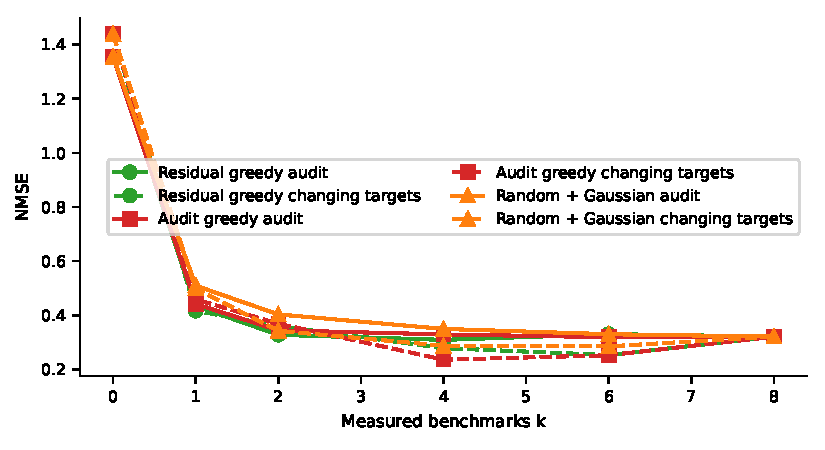
\includegraphics[width=\linewidth]{../artifacts/target_support.pdf}
\caption{Original MTEB dense error with fixed audit targets (solid) and policy-dependent observed unacquired panel targets (dashed). Dashed curves do not share target supports across policies and are not head-to-head evidence of superior transfer. The selector minimizes a sum of conditional variances, whereas plotted error averages over its scored support. Source: \artifact{artifacts/target_support.pdf}.}
\label{fig:target}
\end{figure}
Native residual selection additionally optimizes unavailable full-panel coordinates not included in its observed-support deployment score. In the original organization-native cohorts, 84/210 row appearances have incomplete panels, so this mismatch is exercised rather than purely hypothetical. It does not change the paired fixed-audit definition in \eqref{eq:loss}. No observed-support-aligned objective or effectiveness claim is made from native deployment curves.

\subsection{Synthetic checks and real trace-risk diagnostics}\label{app:synthetic}
\begin{table}[ht]
\centering
\caption{One synthetic Gaussian check, $n=100{,}000$, seven coordinates, targets 4,5,6 (zero-indexed), nested anchors 0--3, RNG seed 20261104. Standard errors are Monte Carlo SEs of mean squared target loss, not leaderboard confidence intervals. Source: \artifact{artifacts/synthetic_identity.csv}; covariance in \artifact{artifacts/synthetic_metadata.json}.}
\label{tab:synthetic}
\begin{tabular}{rrrrr}
\toprule
$k$ & Trace NMSE & Empirical NMSE & MC SE & Absolute discrepancy \\
\midrule
\tableinput{../artifacts/paper_synthetic.tex}
\bottomrule
\end{tabular}
\end{table}
The covariance is formed as $BB^\top+0.4I$ for a seeded $7\times3$ normal matrix and normalized to unit diagonal. The numerical predictor retains its small ridge; the separate rank-one identity check uses exact conditioning. This single well-specified distribution does not validate missingness assumptions, shifted-model prediction, or the estimated trace as a real-data error certificate. \artifact{artifacts/risk_calibration.csv} compares original dense-test errors with fitted traces but contains no predictive interval coverage study.

\section{Implementation details and audit/deviation ledger}\label{app:details}
\paragraph{Task roles and normalization.}
MTEB assigns the audit role when the integer SHA256 of \texttt{audit-role:101:<task>} modulo three equals zero; candidates take the other roles. Ordering uses training coverage and stable hash/panel order. The standard-deviation eligibility floor is $10^{-6}$; retained training cells alone set means/scales. Native eligibility is fixed at the largest plotted $k$, avoiding a different row cohort at each budget. Wide tuning uses native validation observed targets and the same random-anchor core criterion. Pairwise covariance insufficient-overlap flags and PSD repair are retained per run; base original runs have no unsupported pairs, while stress reports reach 11.11\% unsupported entries and 15.64\% relative pre-renormalization PSD repair. Wide-panel repair is nonzero and is reported rather than treated as a guarantee of faithful covariance estimation.

\paragraph{Factor and selector details.}
For a new standardized row, factor prediction uses $u=(B_A^\top B_A+\alpha I)^{-1}B_A^\top z_A$ with task loadings fixed from training. D-optimal acquisition greedily maximizes the loading log-determinant increment, averaged over the three fitted starts; no optimality claim is attached. In addition to original nonconvergence flags, wide MTEB seeds 11,37,53 each have only one converged start out of three at their selected rank-two/ridge-.1 configuration, with the other starts capped at 200. Wide seeds 23,71 and all connected OpenLLM starts are convergence-flagged. Full selection details are in \artifact{artifacts/selected_lowrank.csv}. Gaussian selected lambdas, shared across principal selectors, are in \artifact{artifacts/hyperparameters.csv}. No-shrinkage and mean-filled covariance are explicitly separate audit-selector configurations; the mean/diagonal case returns training means rather than measuring useful labels.

\paragraph{Random paths and validation budgets.}
Random seed is outer seed plus 811, producing 50 independent nested permutations restricted to each row's available candidates. The same path bank enters Gaussian/factor tuning and original headline evaluation; finite-bank sensitivity is therefore conditional on the original fitted choice, not a full retuning study. The second bank is sensitivity only. The global budget heuristic estimates the SE at the validation-minimum $k$ using 500 organization-cluster resamples (seed outer plus 411), then chooses the smallest candidate $k$ within that SE, including zero. Its SE is neither a test interval nor a calibrated individual risk bound. Dense curves include $0,1,2,4,6,8$ for original MTEB and $0,1,2,3$ for OpenLLM. Native original curves end at 4 and 2, respectively; unsupported selected-budget joins are not manufactured.

\paragraph{Training-label deletion.}
For deletion rate $\rho\in\{.2,.5\}$, MCAR has probability $\rho$. Task-propensity weights are $(c_j+.05)^{-1}$ using original training coverage $c_j$; synthetic score-dependent weights are $.1+q_{ij}$ with original within-task training percentile $q_{ij}$. A scalar $a$ is chosen so that $p_{ij}=\min(.95,aw_{ij})$ averages to the requested rate over originally observed cells. An outer-seed-plus-941 uniform draw per cell couples rates. Original training labels may define deletion weights but are inaccessible to preprocessing/fitting after deletion. Test/validation targets and panels stay fixed. The retained-scale normalization changes across conditions, which is why Figure~\ref{fig:missing} uses raw error. No exogenous candidate-availability experiment was run.

\subsection{Audit record and omitted analyses}\label{app:audit}
The independent local protocol audit reconstructed 736,340 original base loss records from 3,454 archived prediction arrays across 20 base runs. Maximum absolute NMSE reconstruction discrepancy was $9.20\times10^{-7}$, consistent with float32 archive precision. It checked available, distinct anchors; never-acquired audits; identical paired target support; identical Gaussian/factor anchors for paired comparisons; flat mean baselines; and training-only fitting/inductive row inference. These are current artifact-consistency checks, not proof of historical independence or external preregistration. Four original synthetic contracts passed; they did not cover every full-runner alias/native-objective issue.

The following deviations remain part of the evidence, not repaired-away inconveniences:
\begin{itemize}
\item Only 1/5 original MTEB organization splits passes the local gate; all five remain descriptive. The planned 62-column intake is not 62-task evaluated target support.
\item Original OpenLLM grouping discarded available SHA/base fields before partitioning. There are 4,451 distinct SHA values among 4,497 retained rows, and 54 duplicate six-score rows beyond the first occurrence. Shared training/test SHA counts are 5,5,4,5,6 in seed order; this does not quantify the sign or size of prediction bias.
\item Organization allocation uses greatest relative row deficit, not the planned sequential cutoff. Task-type round-robin was omitted. Deterministic acquisition ties use panel order, not literal canonical-task ordering. Duplicate training rows are counted, not removed; source evaluator versions were not harmonized.
\item Complete-training-row covariance, the intentionally wrong retained-pre-acquisition-variance diagnostic, and the standardized-variance tie comparator were planned but not implemented. Complete-row covariance was feasible (76--95 training rows in original MTEB manifests), so omission is not called infeasibility. Availability stress, category results, chronological/lineage tests, predictive interval calibration, and further data sources were not run. No strongest-comparator pre-test lock is available; all baselines are reported descriptively.
\item The internal lock hashes the plan, criteria, and manifests, not all processed data, fitted objects, tuning, paths, or budgets with an external timestamp. Two OpenLLM schema-head rows expose score values before locking. No current-code direct test-driven tuning was found, but no sealed-test historical certification is possible.
\item A smoke run was superseded before efficacy analysis to enforce the native fixed-cohort budget ceilings. Its files remain under \artifact{results/smoke_superseded/}; they are not pooled into final tables. The first sensitivity launch failed before fitting because an overlap assertion treated blank SHA keys as identities; the successful rerun consistently ignored empty/whitespace keys while forbidding recorded nonempty overlap. Both logs remain.
\item Cached \texttt{\_done.json} causes unconditional skipping without verifying source/data/configuration identity. Reproductions must use fresh result directories or archive old results; fresh hashes cannot retrospectively establish a pre-test lock.
\end{itemize}
Exact source audit and chronology: \artifact{audit_protocol.md}, \artifact{experiment_log.md}, \artifact{protocol/sensitivity_plan.md}, \artifact{sensitivity_runs.log}, and \artifact{sensitivity_runs_v2.log}. The sensitivities were specified after original predictions and before their own efficacy evaluation; they are not external preregistration or untouched confirmation.

\section{Reproducibility, resources, and source records}\label{app:repro}
All paths below are relative to the workspace root \texttt{/work}. This manuscript was assembled from existing experiments; no experimental implementation or efficacy rerun was performed for manuscript drafting. The deliverable is an anonymous-format research artifact, not a statement of conference acceptance or submission.

\subsection{Environment, commands, and artifact mapping}
The numerical environment records Python 3.11.15 on Linux x86\_64/glibc 2.41, CPU-only execution, 40 logical CPUs visible, and one BLAS/OpenMP thread per process. Direct pins are NumPy 2.4.6, SciPy 1.17.1, pandas 3.0.6, scikit-learn 1.9.1, PyArrow 26.0.1, Matplotlib 3.11.2, requests 2.34.2, and pytest 9.2.0; full installed pins are in \artifact{requirements.lock}. No GPU or paid API is needed for score-table experiments. CPU hardware model and complete per-run memory traces were not recorded in \artifact{environment.json}; a manuscript-stage \texttt{lscpu} inventory records Intel Xeon Gold 6230 at 2.10 GHz (\artifact{paper/hardware.txt}), not a historical worker-allocation log. A logical-CPU count is not a measured allocation of 40 workers.

The following existing commands reproduce the numerical pipeline; they are documented commands, not manuscript-stage reruns. Run from \texttt{/work}, using a fresh result location or archiving previous \texttt{results/} before a true rerun because cache skips do not validate provenance.
\begin{verbatim}
python -m pip install -r requirements.txt
export OPENBLAS_NUM_THREADS=1 OMP_NUM_THREADS=1 CUDA_VISIBLE_DEVICES=''
python src/data.py
python src/cohorts.py
python -m pytest -q
python src/run.py
python src/run.py --stress
python src/sensitivity.py
python src/theory_check.py
python src/diagnostics.py
python src/mc_sensitivity.py
python src/reproduce_check.py
python src/analyze.py
python src/manuscript_tables.py
latexmk -pdf -interaction=nonstopmode -halt-on-error -cd paper/main.tex
cp paper/main.pdf paper.pdf
\end{verbatim}
The data command downloads pinned sources; it does not run language/embedding models. Shell reproduction assumes access and appropriate use rights for those sources. The raw score inputs are existing evaluations, not newly evaluated examples. Public archive retrieval depends on source availability; source SHA256/provenance records should be checked rather than trusting a cache sentinel.

\begin{table}[ht]
\centering
\caption{Evidence-to-artifact map. Analysis tables and figures are generated from stored loss files by \texttt{src/analyze.py}; no handwritten efficacy output substitutes for the CSVs.}
\label{tab:map}
\begin{tabular}{p{.35\linewidth}p{.58\linewidth}}
\toprule
Evidence & Authoritative local path \\
\midrule
Source versions and masks & \path{data/processed/mteb_provenance.csv}; \path{protocol/manifests.json}; \path{protocol/sensitivity_manifests.json} \\
Core and fixed-budget errors/CIs & \path{artifacts/summary.csv}; \path{artifacts/main_table.tex}; \path{artifacts/contrast_table.tex} \\
Cohorts and split estimates & \path{artifacts/cohort_counts.csv}; \path{artifacts/sensitivity_cohorts.csv}; \path{artifacts/split_results.csv} \\
Validation budgets and fits & \path{artifacts/validation_budgets.csv}; \path{artifacts/selected_lowrank.csv}; \path{artifacts/hyperparameters.csv} \\
Figures~\ref{fig:budgets},\ref{fig:missing},\ref{fig:target} & \path{artifacts/budget_curves.pdf}; \path{artifacts/missingness.pdf}; \path{artifacts/target_support.pdf} \\
Numerical and risk diagnostics & \path{artifacts/synthetic_identity.csv}; \path{artifacts/risk_calibration.csv}; \path{artifacts/random_bank_mc.csv}; \path{artifacts/random_bank_sensitivity.csv} \\
Reproduction/resources & \path{artifacts/reproduction_check.json}; \path{artifacts/run_resources.csv}; \path{environment.json}; \path{requirements.lock} \\
\bottomrule
\end{tabular}
\end{table}
Filter \artifact{artifacts/summary.csv} by \texttt{regime=organization}, \texttt{budget=core}, and $(\texttt{dataset},\texttt{condition},\texttt{cohort})$ equal to $(\texttt{mteb},\texttt{base},\texttt{dense})$, $(\texttt{mteb},\texttt{wide\_native},\texttt{native})$, $(\texttt{openllm},\texttt{base},\texttt{dense})$, or $(\texttt{openllm},\texttt{alias\_connected},\texttt{dense})$ for the four full-table columns. Do not pool native/dense appearances or superseded smoke output. Base/sensitivity archives include truth, training means/scales, anchor indices, row IDs, and predictions; stress runs retain losses/validation logs but not full prediction archives. Redistribution restrictions apply to row-level OpenLLM derivatives.

\subsection{Measured resources and incomplete accounting}\label{app:resources}
The 48 stored pipeline timings total 516.70 wall seconds: 20 original pipelines, 18 training-deletion pipelines, and ten sensitivity pipelines. Original MTEB pipelines range 3.59--4.22 seconds, original OpenLLM 21.88--23.35 seconds; wide MTEB 24.68--28.87 seconds and connected OpenLLM 11.82--26.94 seconds. Stress pipelines each take approximately 0.25--0.31 seconds. These timings cover stored fitting/evaluation procedures, not acquisition of new whole-benchmark labels. Training fitting is small-matrix CPU work; pairwise covariance scales roughly as $O(nd^2)$, while repeated factor fits, design solves, and resampling add overhead. No general end-to-end speedup is measured.

A separate original MTEB organization-seed-11 reproduction has exact CSV agreement for 3,520 records, 3.514 wall seconds, 5.273 user CPU seconds, 0.115 system CPU seconds, and peak RSS 157,672 KiB (Linux). This one-run memory measurement is not a full-project memory maximum. The source archive is approximately 377 MiB (396 decimal MB) compressed and was streamed rather than expanded; raw benchmark datasets and weights are not downloaded. The request imposed a 5 GB storage ceiling; a manuscript-stage regular-file apparent-size inventory records 870,484,414 bytes, not a historical storage peak (\artifact{paper/storage.txt}).

Resource totals do not include all acquisition, analysis/bootstrap, preliminary/superseded, failed-launch, writing-agent, or LaTeX costs. Full-project compute and every pipeline's peak memory are unavailable; these omissions are not presented as zero. The current hardware/storage inventories cannot reconstruct historical peaks or certify project-wide resource use. Existing per-run timings, logs, and the reproduction check remain the quantitative experiment resource evidence.

\subsection{Asset versions, access, and licenses}\label{app:assets}
The preserved MTEB source is
\begin{quote}\url{https://github.com/embeddings-benchmark/results}\end{quote}
with immutable commit \texttt{6dabbcc68c28ea5f180ce7df79347b3ca9cc6383}; the direct archive endpoint is
\begin{quote}\url{https://codeload.github.com/embeddings-benchmark/results/tar.gz/6dabbcc68c28ea5f180ce7df79347b3ca9cc6383}.\end{quote}
The result metadata are CC0-1.0 according to the supplied provenance; this does not license upstream datasets or model weights. The preserved OpenLLM source is
\begin{quote}\url{https://huggingface.co/datasets/open-llm-leaderboard/contents}\end{quote}
at commit \texttt{9c09a7cae43334062a82cb164f2ef255013dafa2}. The exact tree endpoint used to identify its single parquet was
\begin{quote}\url{https://huggingface.co/api/datasets/open-llm-leaderboard/contents/tree/9c09a7cae43334062a82cb164f2ef255013dafa2?recursive=true}.\end{quote}
The preserved source-byte SHA256 values are:
\begin{flushleft}
MTEB archive:\\
\texttt{84773e577197630206eacc1790c5fd793d21393b698f6562b0a8f0a1ea31002f}\\
OpenLLM parquet:\\
\texttt{f13a7061e63133bc8745d89f8c7a56148584940ede22d3b27e21cad1e078dca5}.
\end{flushleft}
See \artifact{data_acquisition.log} and \artifact{data/processed/openllm_schema.json}. Its data license is unspecified. Public accessibility and individual model Hub License values do not resolve score-table redistribution rights. The local analysis used public records without accounts; no claim of full license/terms verification is made. Original code is MIT-licensed per \artifact{LICENSE}; third-party packages and the official template retain their own terms. The release policy in \artifact{DATA_LICENSES.md} excludes raw OpenLLM parquet/CSV and per-model prediction/loss archives from public distribution. Source PDFs are local reading references, not redistributed as newly licensed assets.

\subsection{Restricted reading and official formatting provenance}\label{app:sources}
Literature access used only the exact five supplied starter bodies, without topical searches, citation graphs, downstream-paper searches, bibliography reading, or attempts to identify unspecified prohibited work. No recognized forbidden exposure was recorded; this is not a claim to have identified or screened all unknown forbidden material. Only selected sections were inspected, not entire papers or proofs; Appendix tables do not invent external results. Exact reading scope, versions known/unknown, UTC requests, byte counts, and hashes are preserved in \artifact{literature/reading_notes.md}, \artifact{literature/sources.md}, and \artifact{literature/access_log.md}. Four arXiv versions remain unverified; Sloth explicitly identifies v5, 1 December 2025. Bibliographic years follow the initial arXiv identifier year, not inferred proceedings metadata.

The exact recorded paper PDF URLs, all accessed 2026-11-04 UTC, are:
\begin{itemize}
\item \url{https://export.arxiv.org/pdf/2210.07316} (18:13:58 UTC).
\item \url{https://export.arxiv.org/pdf/2402.14992} (18:14:03 UTC).
\item \url{https://export.arxiv.org/pdf/2407.12844} (18:14:09 UTC).
\item \url{https://export.arxiv.org/pdf/2405.10938} (18:14:13 UTC).
\item \url{https://export.arxiv.org/pdf/2412.06540} (18:14:18 UTC).
\end{itemize}
These URLs were HTTP 200. The official formatting/rules records, separate from scientific references, are:
\begin{itemize}
\item \url{https://neurips.cc/Conferences/2026/PaperInformation/StyleFiles}, 18:18:40 UTC: HTTP 404, no redirect followed.
\item \url{https://neurips.cc/Conferences/2026/CallForPapers}, 18:18:42 UTC: HTTP 200.
\item \url{https://media.neurips.cc/Conferences/NeurIPS2026/Formatting_Instructions_For_NeurIPS_2026.zip}, 18:19:15 UTC: HTTP 200.
\item \url{https://neurips.cc/Conferences/2026/MainTrackHandbook}, 18:19:17 UTC: HTTP 200.
\end{itemize}
The official 2026 style declares revision 2026-01-29. Its unmodified archive SHA256 is \texttt{82473931e3ef710fcd3f4a8cd4119b9de32e56825f90f9e5a6d55f2d01b817d9}. Anonymous main-track default formatting is used without margin/style changes, no acknowledgments, and no \texttt{final} or \texttt{preprint} option. Main-track instructions permit nine content pages before references, with technical appendices and the required 16-topic checklist in the same PDF. Official originals remain in \artifact{paper/neurips2026/}; the filled checklist is a separate copy retaining official questions and guidelines. Formatting a research artifact this way does not mean it has been accepted or submitted.

\clearpage
\section*{NeurIPS Paper Checklist}




\begin{enumerate}

\item {\bf Claims}
    \item[] Question: Do the main claims made in the abstract and introduction accurately reflect the paper's contributions and scope?
    \item[] Answer: \answerYes{} % Replace by \answerYes{}, \answerNo{}, or \answerNA{}.
    \item[] Justification: The abstract and Sections~\ref{sec:intro} and~\ref{sec:results} state the failed feasibility gate, descriptive status, limited task support, and distinct post-audit sensitivities; no algorithmic novelty or confirmed superiority is claimed.
    \item[] Guidelines:
    \begin{itemize}
        \item The answer \answerNA{} means that the abstract and introduction do not include the claims made in the paper.
        \item The abstract and/or introduction should clearly state the claims made, including the contributions made in the paper and important assumptions and limitations. A \answerNo{} or \answerNA{} answer to this question will not be perceived well by the reviewers. 
        \item The claims made should match theoretical and experimental results, and reflect how much the results can be expected to generalize to other settings. 
        \item It is fine to include aspirational goals as motivation as long as it is clear that these goals are not attained by the paper. 
    \end{itemize}

\item {\bf Limitations}
    \item[] Question: Does the paper discuss the limitations of the work performed by the authors?
    \item[] Answer: \answerYes{} % Replace by \answerYes{}, \answerNo{}, or \answerNA{}.
    \item[] Justification: Section~\ref{sec:discussion} and Appendix~\ref{app:audit} discuss coverage selection, dependence, exposure history, covariance assumptions, omitted ablations, and bounded low-rank convergence.
    \item[] Guidelines:
    \begin{itemize}
        \item The answer \answerNA{} means that the paper has no limitation while the answer \answerNo{} means that the paper has limitations, but those are not discussed in the paper. 
        \item The authors are encouraged to create a separate ``Limitations'' section in their paper.
        \item The paper should point out any strong assumptions and how robust the results are to violations of these assumptions (e.g., independence assumptions, noiseless settings, model well-specification, asymptotic approximations only holding locally). The authors should reflect on how these assumptions might be violated in practice and what the implications would be.
        \item The authors should reflect on the scope of the claims made, e.g., if the approach was only tested on a few datasets or with a few runs. In general, empirical results often depend on implicit assumptions, which should be articulated.
        \item The authors should reflect on the factors that influence the performance of the approach. For example, a facial recognition algorithm may perform poorly when image resolution is low or images are taken in low lighting. Or a speech-to-text system might not be used reliably to provide closed captions for online lectures because it fails to handle technical jargon.
        \item The authors should discuss the computational efficiency of the proposed algorithms and how they scale with dataset size.
        \item If applicable, the authors should discuss possible limitations of their approach to address problems of privacy and fairness.
        \item While the authors might fear that complete honesty about limitations might be used by reviewers as grounds for rejection, a worse outcome might be that reviewers discover limitations that aren't acknowledged in the paper. The authors should use their best judgment and recognize that individual actions in favor of transparency play an important role in developing norms that preserve the integrity of the community. Reviewers will be specifically instructed to not penalize honesty concerning limitations.
    \end{itemize}

\item {\bf Theory assumptions and proofs}
    \item[] Question: For each theoretical result, does the paper provide the full set of assumptions and a complete (and correct) proof?
    \item[] Answer: \answerYes{} % Replace by \answerYes{}, \answerNo{}, or \answerNA{}.
    \item[] Justification: Section~\ref{sec:theory} states finite positive-definite Gaussian and exact-observation assumptions; Appendix~\ref{app:proofs} supplies full proofs and counterexamples, without an empirical generalization guarantee.
    \item[] Guidelines:
    \begin{itemize}
        \item The answer \answerNA{} means that the paper does not include theoretical results. 
        \item All the theorems, formulas, and proofs in the paper should be numbered and cross-referenced.
        \item All assumptions should be clearly stated or referenced in the statement of any theorems.
        \item The proofs can either appear in the main paper or the supplemental material, but if they appear in the supplemental material, the authors are encouraged to provide a short proof sketch to provide intuition. 
        \item Inversely, any informal proof provided in the core of the paper should be complemented by formal proofs provided in appendix or supplemental material.
        \item Theorems and Lemmas that the proof relies upon should be properly referenced. 
    \end{itemize}

    \item {\bf Experimental result reproducibility}
    \item[] Question: Does the paper fully disclose all the information needed to reproduce the main experimental results of the paper to the extent that it affects the main claims and/or conclusions of the paper (regardless of whether the code and data are provided or not)?
    \item[] Answer: \answerYes{} % Replace by \answerYes{}, \answerNo{}, or \answerNA{}.
    \item[] Justification: Sections~\ref{sec:protocol}--\ref{sec:results} and Appendix~\ref{app:repro} specify pinned inputs, extraction, splits, tuning, metrics, uncertainty, commands, and artifact mappings. Historical test sealing and external preregistration are explicitly not certified.
    \item[] Guidelines:
    \begin{itemize}
        \item The answer \answerNA{} means that the paper does not include experiments.
        \item If the paper includes experiments, a \answerNo{} answer to this question will not be perceived well by the reviewers: Making the paper reproducible is important, regardless of whether the code and data are provided or not.
        \item If the contribution is a dataset and\slash or model, the authors should describe the steps taken to make their results reproducible or verifiable. 
        \item Depending on the contribution, reproducibility can be accomplished in various ways. For example, if the contribution is a novel architecture, describing the architecture fully might suffice, or if the contribution is a specific model and empirical evaluation, it may be necessary to either make it possible for others to replicate the model with the same dataset, or provide access to the model. In general. releasing code and data is often one good way to accomplish this, but reproducibility can also be provided via detailed instructions for how to replicate the results, access to a hosted model (e.g., in the case of a large language model), releasing of a model checkpoint, or other means that are appropriate to the research performed.
        \item While NeurIPS does not require releasing code, the conference does require all submissions to provide some reasonable avenue for reproducibility, which may depend on the nature of the contribution. For example
        \begin{enumerate}
            \item If the contribution is primarily a new algorithm, the paper should make it clear how to reproduce that algorithm.
            \item If the contribution is primarily a new model architecture, the paper should describe the architecture clearly and fully.
            \item If the contribution is a new model (e.g., a large language model), then there should either be a way to access this model for reproducing the results or a way to reproduce the model (e.g., with an open-source dataset or instructions for how to construct the dataset).
            \item We recognize that reproducibility may be tricky in some cases, in which case authors are welcome to describe the particular way they provide for reproducibility. In the case of closed-source models, it may be that access to the model is limited in some way (e.g., to registered users), but it should be possible for other researchers to have some path to reproducing or verifying the results.
        \end{enumerate}
    \end{itemize}


\item {\bf Open access to data and code}
    \item[] Question: Does the paper provide open access to the data and code, with sufficient instructions to faithfully reproduce the main experimental results, as described in supplemental material?
    \item[] Answer: \answerNo{} % Replace by \answerYes{}, \answerNo{}, or \answerNA{}.
    \item[] Justification: The local deliverable contains code, commands, manifests, and aggregate artifacts (Appendix~\ref{app:repro}), but no verified public anonymous release URL is available. Raw and row-level OpenLLM data are not redistributed because its dataset license is unresolved.
    \item[] Guidelines:
    \begin{itemize}
        \item The answer \answerNA{} means that paper does not include experiments requiring code.
        \item Please see the NeurIPS code and data submission guidelines (\url{https://neurips.cc/public/guides/CodeSubmissionPolicy}) for more details.
        \item While we encourage the release of code and data, we understand that this might not be possible, so \answerNo{} is an acceptable answer. Papers cannot be rejected simply for not including code, unless this is central to the contribution (e.g., for a new open-source benchmark).
        \item The instructions should contain the exact command and environment needed to run to reproduce the results. See the NeurIPS code and data submission guidelines (\url{https://neurips.cc/public/guides/CodeSubmissionPolicy}) for more details.
        \item The authors should provide instructions on data access and preparation, including how to access the raw data, preprocessed data, intermediate data, and generated data, etc.
        \item The authors should provide scripts to reproduce all experimental results for the new proposed method and baselines. If only a subset of experiments are reproducible, they should state which ones are omitted from the script and why.
        \item At submission time, to preserve anonymity, the authors should release anonymized versions (if applicable).
        \item Providing as much information as possible in supplemental material (appended to the paper) is recommended, but including URLs to data and code is permitted.
    \end{itemize}


\item {\bf Experimental setting/details}
    \item[] Question: Does the paper specify all the training and test details (e.g., data splits, hyperparameters, how they were chosen, type of optimizer) necessary to understand the results?
    \item[] Answer: \answerYes{} % Replace by \answerYes{}, \answerNo{}, or \answerNA{}.
    \item[] Justification: Sections~\ref{sec:protocol} and~\ref{sec:method} specify the holdouts, task roles, preprocessing, hyperparameter grids, and masked-factor optimization; Appendix~\ref{app:details} gives remaining details.
    \item[] Guidelines:
    \begin{itemize}
        \item The answer \answerNA{} means that the paper does not include experiments.
        \item The experimental setting should be presented in the core of the paper to a level of detail that is necessary to appreciate the results and make sense of them.
        \item The full details can be provided either with the code, in appendix, or as supplemental material.
    \end{itemize}

\item {\bf Experiment statistical significance}
    \item[] Question: Does the paper report error bars suitably and correctly defined or other appropriate information about the statistical significance of the experiments?
    \item[] Answer: \answerYes{} % Replace by \answerYes{}, \answerNo{}, or \answerNA{}.
    \item[] Justification: Section~\ref{sec:uncertainty} defines 2,000 paired cluster-bootstrap percentile intervals conditional on fixed pipelines, cohorts, and the original random bank. They are descriptive intervals, not multiplicity-corrected superiority tests or predictive intervals.
    \item[] Guidelines:
    \begin{itemize}
        \item The answer \answerNA{} means that the paper does not include experiments.
        \item The authors should answer \answerYes{} if the results are accompanied by error bars, confidence intervals, or statistical significance tests, at least for the experiments that support the main claims of the paper.
        \item The factors of variability that the error bars are capturing should be clearly stated (for example, train/test split, initialization, random drawing of some parameter, or overall run with given experimental conditions).
        \item The method for calculating the error bars should be explained (closed form formula, call to a library function, bootstrap, etc.)
        \item The assumptions made should be given (e.g., Normally distributed errors).
        \item It should be clear whether the error bar is the standard deviation or the standard error of the mean.
        \item It is OK to report 1-sigma error bars, but one should state it. The authors should preferably report a 2-sigma error bar than state that they have a 96\% CI, if the hypothesis of Normality of errors is not verified.
        \item For asymmetric distributions, the authors should be careful not to show in tables or figures symmetric error bars that would yield results that are out of range (e.g., negative error rates).
        \item If error bars are reported in tables or plots, the authors should explain in the text how they were calculated and reference the corresponding figures or tables in the text.
    \end{itemize}

\item {\bf Experiments compute resources}
    \item[] Question: For each experiment, does the paper provide sufficient information on the computer resources (type of compute workers, memory, time of execution) needed to reproduce the experiments?
    \item[] Answer: \answerNo{} % Replace by \answerYes{}, \answerNo{}, or \answerNA{}.
    \item[] Justification: Appendix~\ref{app:resources} reports CPU environment, all 48 stored pipeline wall times, and a measured reproduction memory check, but complete project-wide compute and per-run peak memory were not recorded. Preliminary, failed, acquisition, and analysis costs are not claimed to be included in those totals.
    \item[] Guidelines:
    \begin{itemize}
        \item The answer \answerNA{} means that the paper does not include experiments.
        \item The paper should indicate the type of compute workers CPU or GPU, internal cluster, or cloud provider, including relevant memory and storage.
        \item The paper should provide the amount of compute required for each of the individual experimental runs as well as estimate the total compute. 
        \item The paper should disclose whether the full research project required more compute than the experiments reported in the paper (e.g., preliminary or failed experiments that didn't make it into the paper). 
    \end{itemize}
    
\item {\bf Code of ethics}
    \item[] Question: Does the research conducted in the paper conform, in every respect, with the NeurIPS Code of Ethics \url{https://neurips.cc/public/EthicsGuidelines}?
    \item[] Answer: \answerNA{} % Replace by \answerYes{}, \answerNo{}, or \answerNA{}.
    \item[] Justification: The separate linked NeurIPS Code of Ethics was not independently reviewed under the restricted access protocol; full conformity is therefore not certified. Section~\ref{sec:ethics} documents impacts, licensing uncertainty, and safeguards without asserting such certification.
    \item[] Guidelines:
    \begin{itemize}
        \item The answer \answerNA{} means that the authors have not reviewed the NeurIPS Code of Ethics.
        \item If the authors answer \answerNo, they should explain the special circumstances that require a deviation from the Code of Ethics.
        \item The authors should make sure to preserve anonymity (e.g., if there is a special consideration due to laws or regulations in their jurisdiction).
    \end{itemize}


\item {\bf Broader impacts}
    \item[] Question: Does the paper discuss both potential positive societal impacts and negative societal impacts of the work performed?
    \item[] Answer: \answerYes{} % Replace by \answerYes{}, \answerNo{}, or \answerNA{}.
    \item[] Justification: Section~\ref{sec:ethics} discusses lower barriers to exploratory evaluation alongside benchmark blind spots and overconfidence; it recommends direct safety-critical evaluation rather than predicted-score certification.
    \item[] Guidelines:
    \begin{itemize}
        \item The answer \answerNA{} means that there is no societal impact of the work performed.
        \item If the authors answer \answerNA{} or \answerNo, they should explain why their work has no societal impact or why the paper does not address societal impact.
        \item Examples of negative societal impacts include potential malicious or unintended uses (e.g., disinformation, generating fake profiles, surveillance), fairness considerations (e.g., deployment of technologies that could make decisions that unfairly impact specific groups), privacy considerations, and security considerations.
        \item The conference expects that many papers will be foundational research and not tied to particular applications, let alone deployments. However, if there is a direct path to any negative applications, the authors should point it out. For example, it is legitimate to point out that an improvement in the quality of generative models could be used to generate Deepfakes for disinformation. On the other hand, it is not needed to point out that a generic algorithm for optimizing neural networks could enable people to train models that generate Deepfakes faster.
        \item The authors should consider possible harms that could arise when the technology is being used as intended and functioning correctly, harms that could arise when the technology is being used as intended but gives incorrect results, and harms following from (intentional or unintentional) misuse of the technology.
        \item If there are negative societal impacts, the authors could also discuss possible mitigation strategies (e.g., gated release of models, providing defenses in addition to attacks, mechanisms for monitoring misuse, mechanisms to monitor how a system learns from feedback over time, improving the efficiency and accessibility of ML).
    \end{itemize}
    
\item {\bf Safeguards}
    \item[] Question: Does the paper describe safeguards that have been put in place for responsible release of data or models that have a high risk for misuse (e.g., pre-trained language models, image generators, or scraped datasets)?
    \item[] Answer: \answerNA{} % Replace by \answerYes{}, \answerNo{}, or \answerNA{}.
    \item[] Justification: No new pretrained model, high-risk generative system, or scraped content dataset is released. Section~\ref{sec:ethics} explains the aggregate-only reporting and limits of score prediction.
    \item[] Guidelines:
    \begin{itemize}
        \item The answer \answerNA{} means that the paper poses no such risks.
        \item Released models that have a high risk for misuse or dual-use should be released with necessary safeguards to allow for controlled use of the model, for example by requiring that users adhere to usage guidelines or restrictions to access the model or implementing safety filters. 
        \item Datasets that have been scraped from the Internet could pose safety risks. The authors should describe how they avoided releasing unsafe images.
        \item We recognize that providing effective safeguards is challenging, and many papers do not require this, but we encourage authors to take this into account and make a best faith effort.
    \end{itemize}

\item {\bf Licenses for existing assets}
    \item[] Question: Are the creators or original owners of assets (e.g., code, data, models), used in the paper, properly credited and are the license and terms of use explicitly mentioned and properly respected?
    \item[] Answer: \answerNo{} % Replace by \answerYes{}, \answerNo{}, or \answerNA{}.
    \item[] Justification: Appendix~\ref{app:assets} credits and pins the existing sources and states MTEB CC0-1.0, but the OpenLLM score-table license remains unspecified; model-license fields do not resolve it. No raw OpenLLM source or row-level derivative redistribution permission is inferred.
    \item[] Guidelines:
    \begin{itemize}
        \item The answer \answerNA{} means that the paper does not use existing assets.
        \item The authors should cite the original paper that produced the code package or dataset.
        \item The authors should state which version of the asset is used and, if possible, include a URL.
        \item The name of the license (e.g., CC-BY 4.0) should be included for each asset.
        \item For scraped data from a particular source (e.g., website), the copyright and terms of service of that source should be provided.
        \item If assets are released, the license, copyright information, and terms of use in the package should be provided. For popular datasets, \url{paperswithcode.com/datasets} has curated licenses for some datasets. Their licensing guide can help determine the license of a dataset.
        \item For existing datasets that are re-packaged, both the original license and the license of the derived asset (if it has changed) should be provided.
        \item If this information is not available online, the authors are encouraged to reach out to the asset's creators.
    \end{itemize}

\item {\bf New assets}
    \item[] Question: Are new assets introduced in the paper well documented and is the documentation provided alongside the assets?
    \item[] Answer: \answerYes{} % Replace by \answerYes{}, \answerNo{}, or \answerNA{}.
    \item[] Justification: The local code and aggregate analysis artifacts are documented by README.md, DATA\_LICENSES.md, and the file/command map in Appendix~\ref{app:repro}; there is no new human dataset or language model. This describes the local deliverable, not a verified public release.
    \item[] Guidelines:
    \begin{itemize}
        \item The answer \answerNA{} means that the paper does not release new assets.
        \item Researchers should communicate the details of the dataset\slash code\slash model as part of their submissions via structured templates. This includes details about training, license, limitations, etc. 
        \item The paper should discuss whether and how consent was obtained from people whose asset is used.
        \item At submission time, remember to anonymize your assets (if applicable). You can either create an anonymized URL or include an anonymized zip file.
    \end{itemize}

\item {\bf Crowdsourcing and research with human subjects}
    \item[] Question: For crowdsourcing experiments and research with human subjects, does the paper include the full text of instructions given to participants and screenshots, if applicable, as well as details about compensation (if any)? 
    \item[] Answer: \answerNA{} % Replace by \answerYes{}, \answerNo{}, or \answerNA{}.
    \item[] Justification: The study uses existing public benchmark score tables and has no crowdsourcing, recruited participants, or new human-subject experiments (Section~\ref{sec:ethics}).
    \item[] Guidelines:
    \begin{itemize}
        \item The answer \answerNA{} means that the paper does not involve crowdsourcing nor research with human subjects.
        \item Including this information in the supplemental material is fine, but if the main contribution of the paper involves human subjects, then as much detail as possible should be included in the main paper. 
        \item According to the NeurIPS Code of Ethics, workers involved in data collection, curation, or other labor should be paid at least the minimum wage in the country of the data collector. 
    \end{itemize}

\item {\bf Institutional review board (IRB) approvals or equivalent for research with human subjects}
    \item[] Question: Does the paper describe potential risks incurred by study participants, whether such risks were disclosed to the subjects, and whether Institutional Review Board (IRB) approvals (or an equivalent approval/review based on the requirements of your country or institution) were obtained?
    \item[] Answer: \answerNA{} % Replace by \answerYes{}, \answerNo{}, or \answerNA{}.
    \item[] Justification: No human-subject study or recruitment was conducted; no IRB approval is claimed (Section~\ref{sec:ethics}).
    \item[] Guidelines:
    \begin{itemize}
        \item The answer \answerNA{} means that the paper does not involve crowdsourcing nor research with human subjects.
        \item Depending on the country in which research is conducted, IRB approval (or equivalent) may be required for any human subjects research. If you obtained IRB approval, you should clearly state this in the paper. 
        \item We recognize that the procedures for this may vary significantly between institutions and locations, and we expect authors to adhere to the NeurIPS Code of Ethics and the guidelines for their institution. 
        \item For initial submissions, do not include any information that would break anonymity (if applicable), such as the institution conducting the review.
    \end{itemize}

\item {\bf Declaration of LLM usage}
    \item[] Question: Does the paper describe the usage of LLMs if it is an important, original, or non-standard component of the core methods in this research? Note that if the LLM is used only for writing, editing, or formatting purposes and does \emph{not} impact the core methodology, scientific rigor, or originality of the research, declaration is not required.
    %this research? 
    \item[] Answer: \answerYes{} % Replace by \answerYes{}, \answerNo{}, or \answerNA{}.
    \item[] Justification: Section~\ref{sec:agents} discloses autonomous LLM-agent participation in research design, implementation, analysis, and drafting. No LLM judge supplies prediction targets, and no new GPU or paid-API experiment was used.
    \item[] Guidelines:
    \begin{itemize}
        \item The answer \answerNA{} means that the core method development in this research does not involve LLMs as any important, original, or non-standard components.
        \item Please refer to our LLM policy in the NeurIPS handbook for what should or should not be described.
    \end{itemize}

\end{enumerate}
\end{document}
